\chapter{Fundamentals}\label{ch:fundamentals}

\begin{chapterabstract}
    In this chapter, we will introduce readers to the fundamentals of federated infrastructure with emphasis on data exchange and see how they compare to centralized architectures.
    The next part will focus directly on Gaia-X as a federated infrastructure representative.
    We will go over its vision, the means to achieve them, their organizational structure and fundamental concepts.
\end{chapterabstract}

\section{Federated Data Infrastructures}\label{sec:federated-data-infrastructures}

Federated infrastructures for data storage are such infrastructures, which do not pool data in a central data store, but instead independent federations of data providers are set up~\cite{otto_federated_2022}.
Instead of relying on a central data silo, data providers publish their offerings in a publicly searchable catalogue along with its metadata, terms and conditions, usage policies, etc.
After consumers find an offer they are interested in, they communicate with the data producer directly (P2P) via a data connector.

The advantages of federated data infrastructures are numerous; they can be more flexible than centralized solutions, which means they could cater to the needs and requirements of more diverse groups of people~\cite{raab_federated_2023}.
Federated architectures can also be more fault resilient than their centralized counterparts as a single node failure doesn't impact the whole network.
Since federated data infrastructures (also called ``Data Spaces'') don't require data to be transferred to a central location, the mere fact that they can be exchanged closer to source can increase data privacy and lower the risk of leaks.

However, the concept of Data Spaces is not without its downsides.
Centralized solutions have the edge over Data Spaces in terms of simplicity; the existence of multiple federations leads to an increased need of interoperability to reduce the increased effort of having to communicate with multiple parties.

\section{About Gaia-X}\label{sec:about-gaia-x}

\textbf{Gaia-X} is the initiative led by the ``Gaia-X Association AISBL'' organization.
The association was registered as an \textit{international non-profit association} \textit{(French: Association Internationale sans but lucratif)} in Belgium in January 2021 and is funded privately.
It was founded by \textit{22} companies and organizations in \textit{January 2021}, but at the time of writing (January 2024), the association has over \textit{350} members from backgrounds like data infrastructure providers, IT startups research institutions and business associations. % TODO: update before completing the thesis
Additionally, representatives from business, politics, academia, research, technology, policy, government, and science from Europe and beyond cooperate with the \textit{Gaia-X Association AISBL} in their mission.
The association claims to have no business interest~\cite{gaiax}.

\section{Goal}\label{sec:gaia-x-goal}

The goal of the \textbf{Gaia-X} initiative is to enable exchange of data and services in a \textit{safe} and \textit{trustworthy} environment~\cite{gaiax}.
The coveted outcome is a federated system connecting many cloud service providers and users together in an environment that is \textit{interoperable} \textit{transparent}, \textit{open}, \textit{secure}, and respects \textit{data rights} and \textit{EU regulations}.

\section{Structure}\label{sec:the-structure}

The organisational structure of the ``Gaia-X Association AISBL'' is well-defined and transparent~\cite{gaiax}.
The topmost body of the \textit{association} is the \textbf{General Assembly}.
It is composed of all the members of the \textit{association} and has complete authority to carry out the objectives of the \textit{Gaia-X initiative}.

Under the \textbf{General Assembly} are the boards \em \textit{Governmental Advisory Board}, \textit{General Advisory Board} and the \textit{Board of Directors}.
The \textbf{Board of Directors} is elected by the \textbf{General Assembly} and is headed by a Chairperson and Vice-Chairperson.
Its purpose is to decide on important matters regarding the \textit{Gaia-X Association}.

Next up is the \textbf{Management Board} and its chairs \em \textit{Policy Rules Committee}, \textit{Data Spaces Business Committee}, and the \textit{Technical Committee}.
Each of the committees also has its own \textit{Working Group}.
The \textbf{Management Board} is appointed by the \textit{Board of Directors} and is composed of the Chief Executive Officer (CEO), the Chief Operating Officer (COO), the Chief Technical Officer (CTO), the Digital Communications Director and the Head of Finance and Administration.
Its purpose is the management of daily activities of \textit{Gaia-X Association}.

\begin{figure}
    \centering
    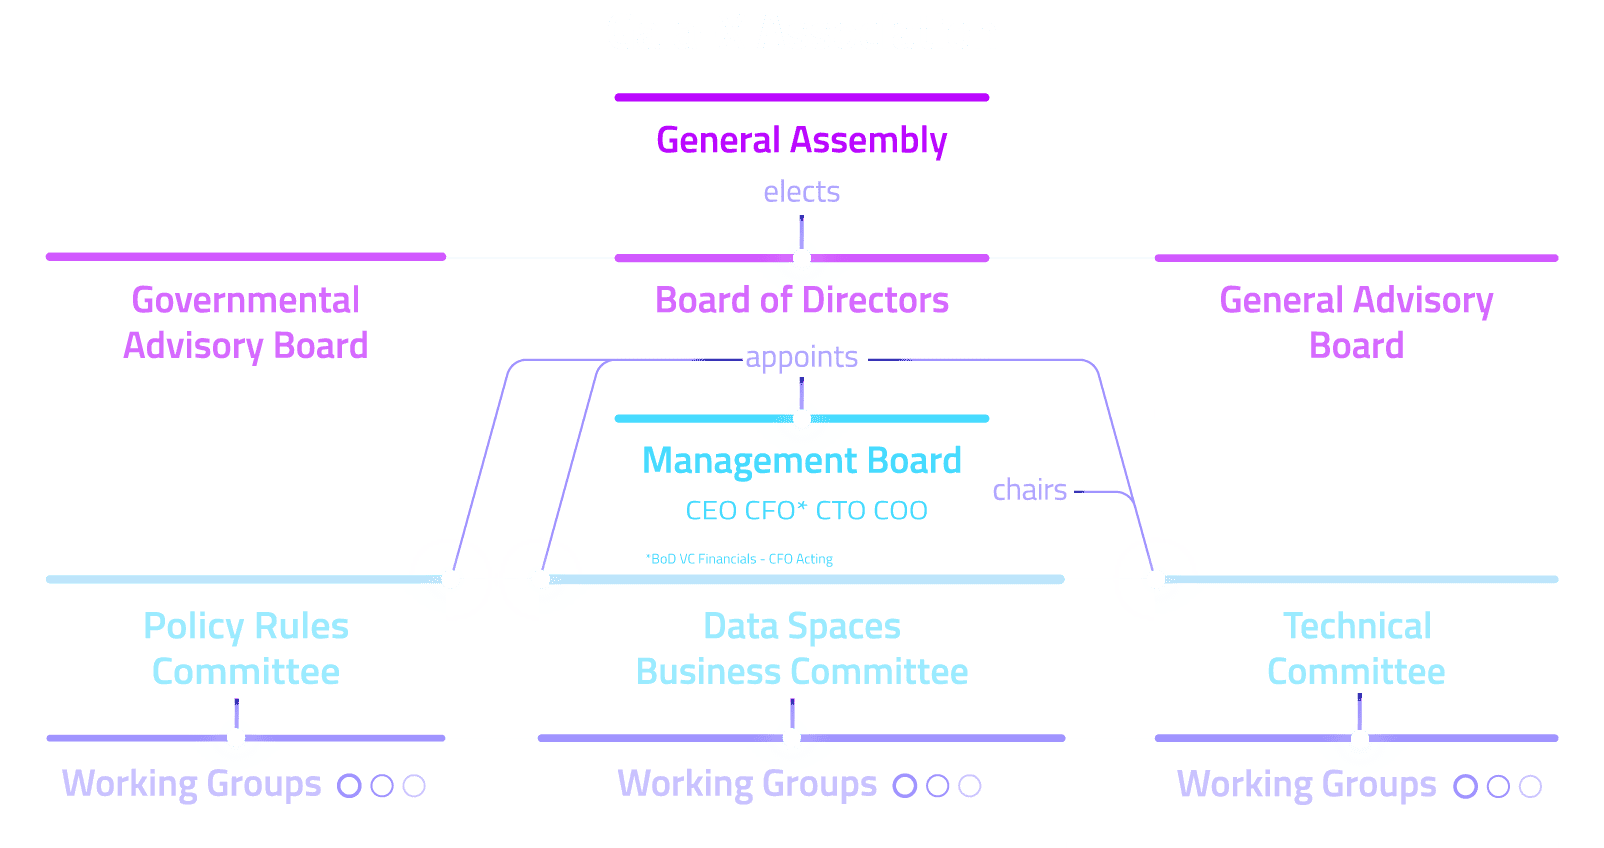
\includegraphics[width=\textwidth]{figures/management-board-structure.png}
    \caption{Organisational structure of the Gaia-X Association~\cite{gaiax}}\label{fig:organisational-board-structure}
\end{figure}

\subsection{Data Spaces Business Committee}\label{subsec:data-spaces-business-committee}

The \textit{Data Spaces Business Committee (DSBC)} focuses on collecting \textit{economic}, \textit{functional}, \textit{operational} and \textit{legal} requirements that facilitate seamless collaboration and interconnection between \textit{Data Spaces}, \textit{Ecosystems}, \textit{Lighthouse Projects\footnote{A lighthouse project is a high-impact, innovative initiative that serves as a model for others, demonstrating leadership and setting a benchmark within an industry or organization.}} and respective \textit{Hubs}~\cite{gaiax}. % FIXME: Data Spaces, Ecosystems, Lighthouse Projects and Hubs not defined yet
Furthermore, the \textit{DSBC} supports the creation of Data Spaces by third parties across Europe and beyond.

\subsection{Policy Rules Committee}\label{subsec:policy-rules-committee}

The \textit{Policy Rules Committee (PRC)} exists to translate the guiding principles of the Gaia-X initiative (\textit{transparency}, \textit{data protection}, \textit{cyber-security}, \textit{portability}, \textit{openness},~\ldots) into High-Level Objectives and to preserve the added value of the \textit{Gaia-X ecosystem}~\cite{gaiax}.
The additional role of the \textit{PRC} is to monitor, integrate and define the relationship with EU regulations and external standards.
The Committee guides and delivers the \textit{Gaia-X Trust Framework}, \textit{Gaia-X Policy Rules and Labelling Document} (formerly Policy Rules Document and Gaia-X Labelling Criteria).
These deliverables are provided by the Committee's three \textit{Working Groups} (WG).
\begin{itemize}
    \item \textbf{Labels \& Qualification} WG:~provides the \textit{Gaia-X Labelling Framework} and prepares the ``Gaia-X Policy Rules and Labelling Document'' together with the \textit{Policy Rules Document} WG
    \item \textbf{Policy Rules Document} WG:~defines \textit{High-Level Objectives} and prepares the ``Gaia-X Policy Rules and Labelling Document'' together with the \textit{Policy Rules Document} WG
    \item \textbf{Compliance} WG:~provides the \textit{Gaia-X Trust Framework}, representing the reference document for the Gaia-X compliance, providing the compulsory set of rules of the Gaia-X Ecosystem
\end{itemize}

\subsection{Technical Committee}\label{subsec:technical-committee}

The purpose of the \textit{Technical Committee (TC)} is to define and implement the technological vision of the \textit{Gaia-X initiative}~\cite{gaiax}.
It is in charge of transforming the high-level objectives of Gaia-X and requirements collected from other Committees and Gaia-X members into the \textit{technology roadmap} and is accountable for its contributors.
The Committee drafts and delivers the Gaia-X \textit{Architecture Document}, \textit{technical specifications} and related \textit{reference implementation}.
These deliverables are provided by the Committee's two \textit{Working Groups} (WG).
\begin{itemize}
    \item \textbf{Architecture} WG:~drafts the ``Gaia-X Architecture Document'', which describes the founding concepts of the \textit{Gaia-X Ecosystem}
    \item \textbf{Service Characteristics} WG:~specifies the Schema for the Self-Descriptions of Providers, their Service Offerings, and the Resources they are composed of
\end{itemize}

\begin{figure}
    \centering
    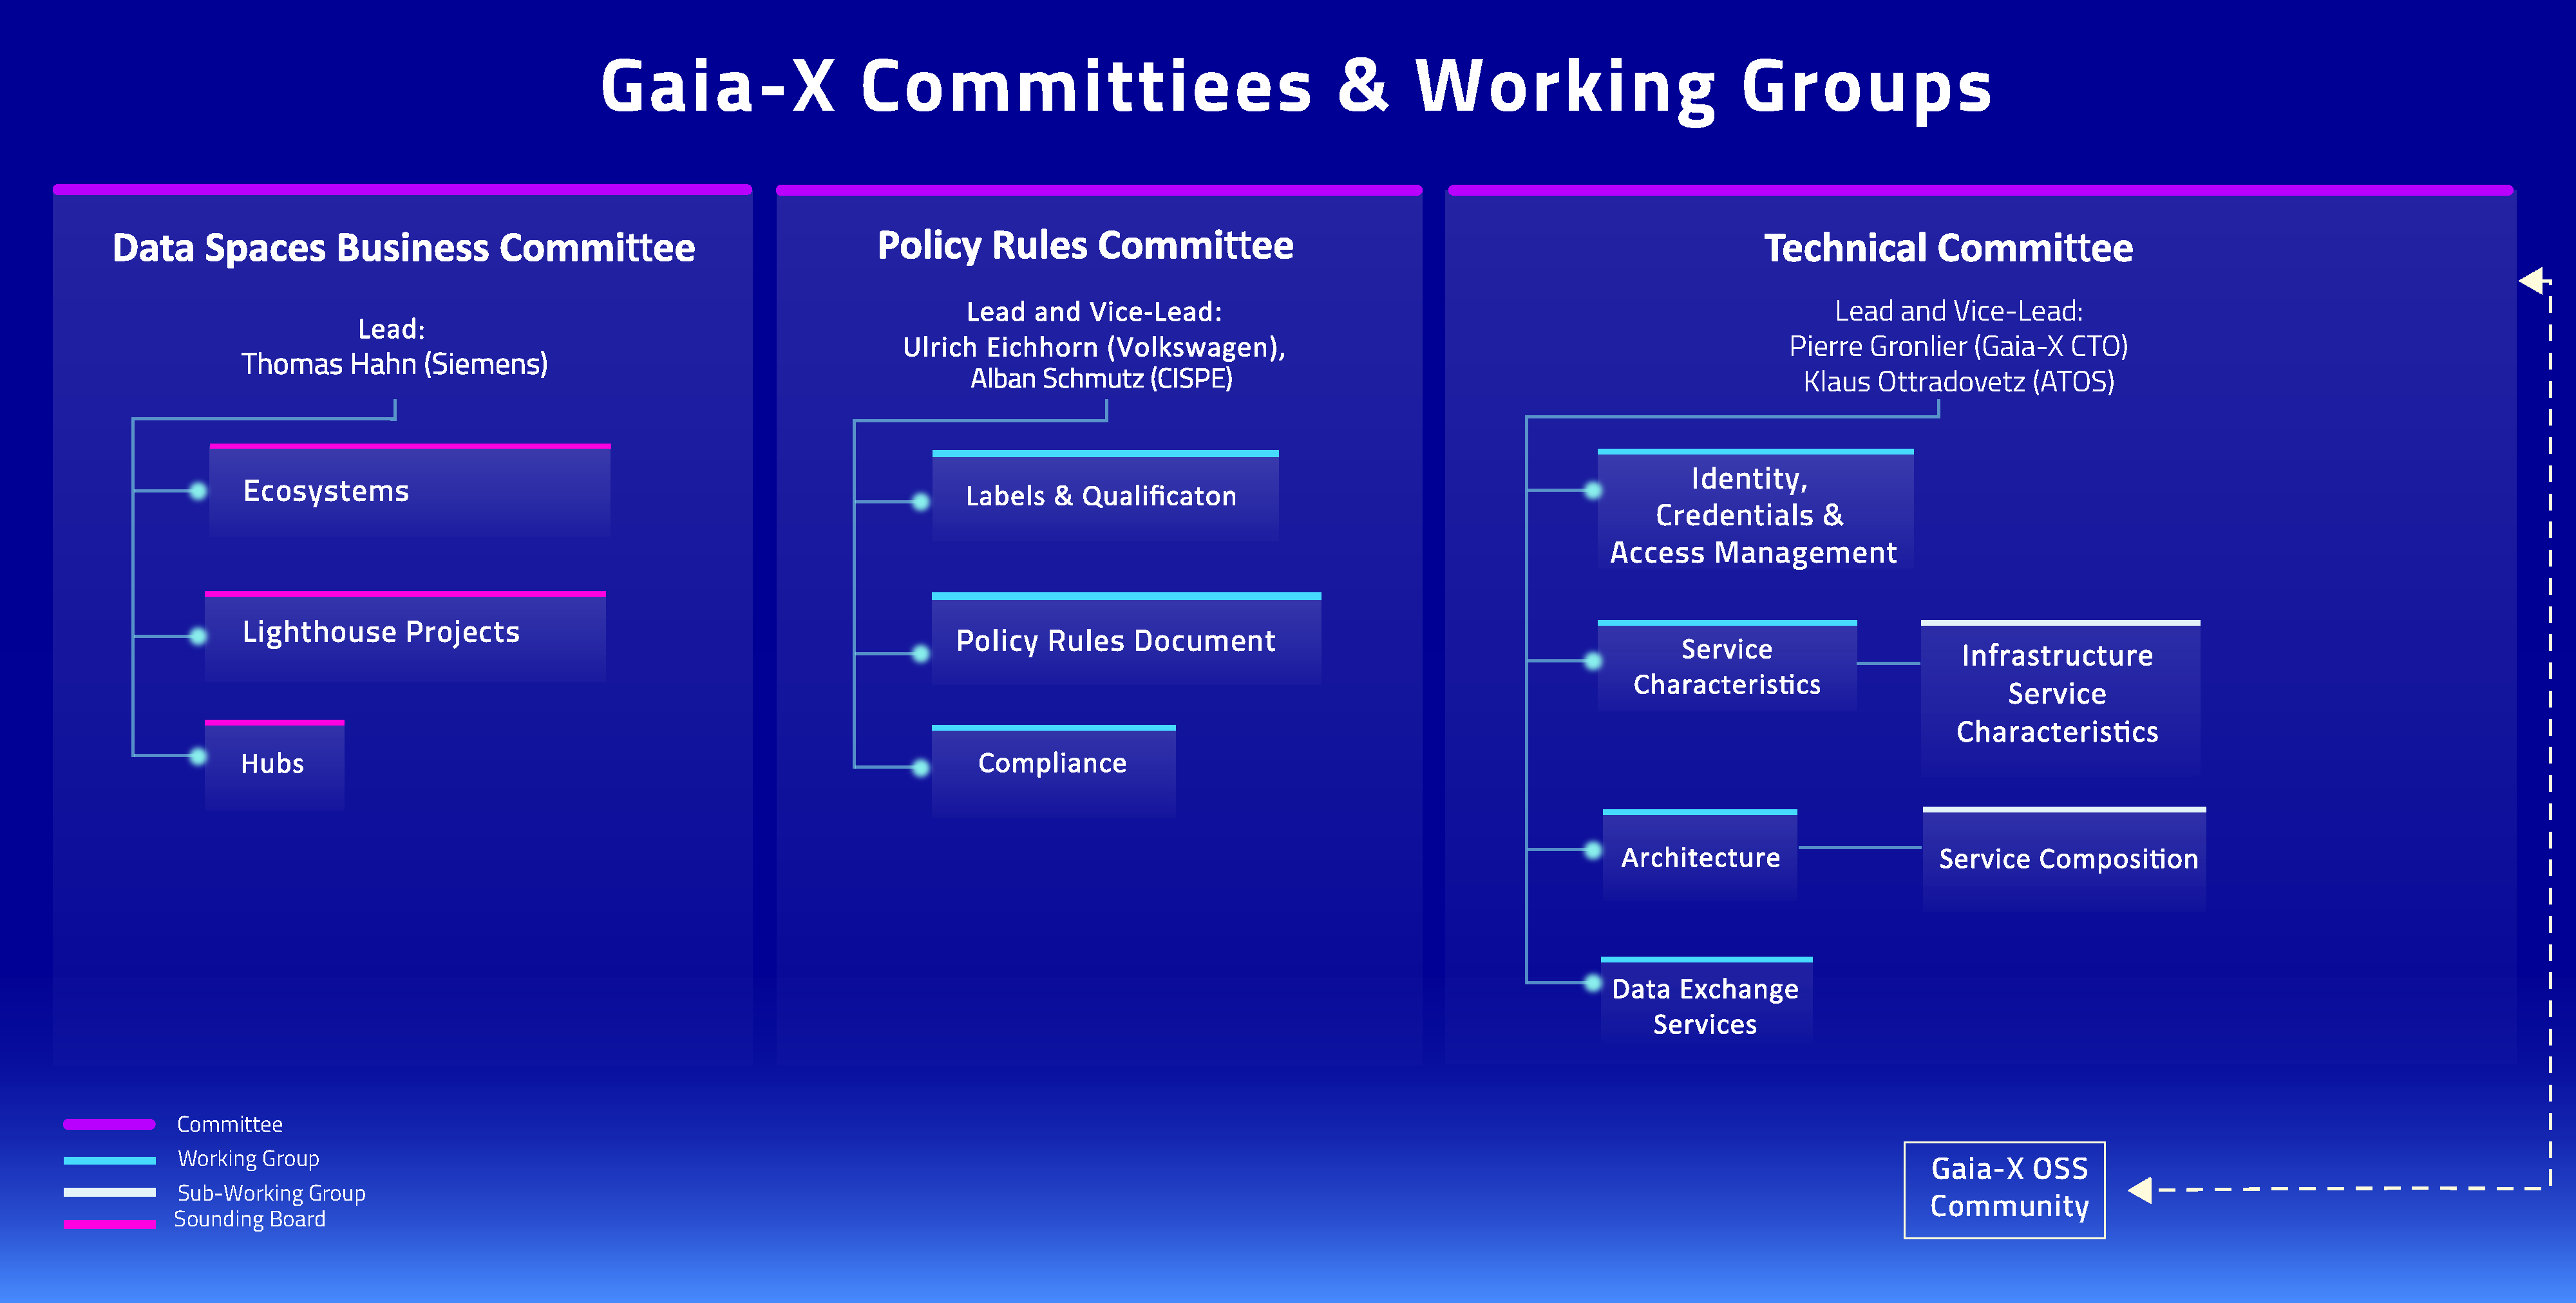
\includegraphics[width=\textwidth]{figures/committees-and-working-groups.pdf}
    \caption{Organisational structure Committees and their Working Groups~\cite{gaiax}}\label{fig:organisational-committees-structure}
\end{figure}

\begin{figure}
    \centering
    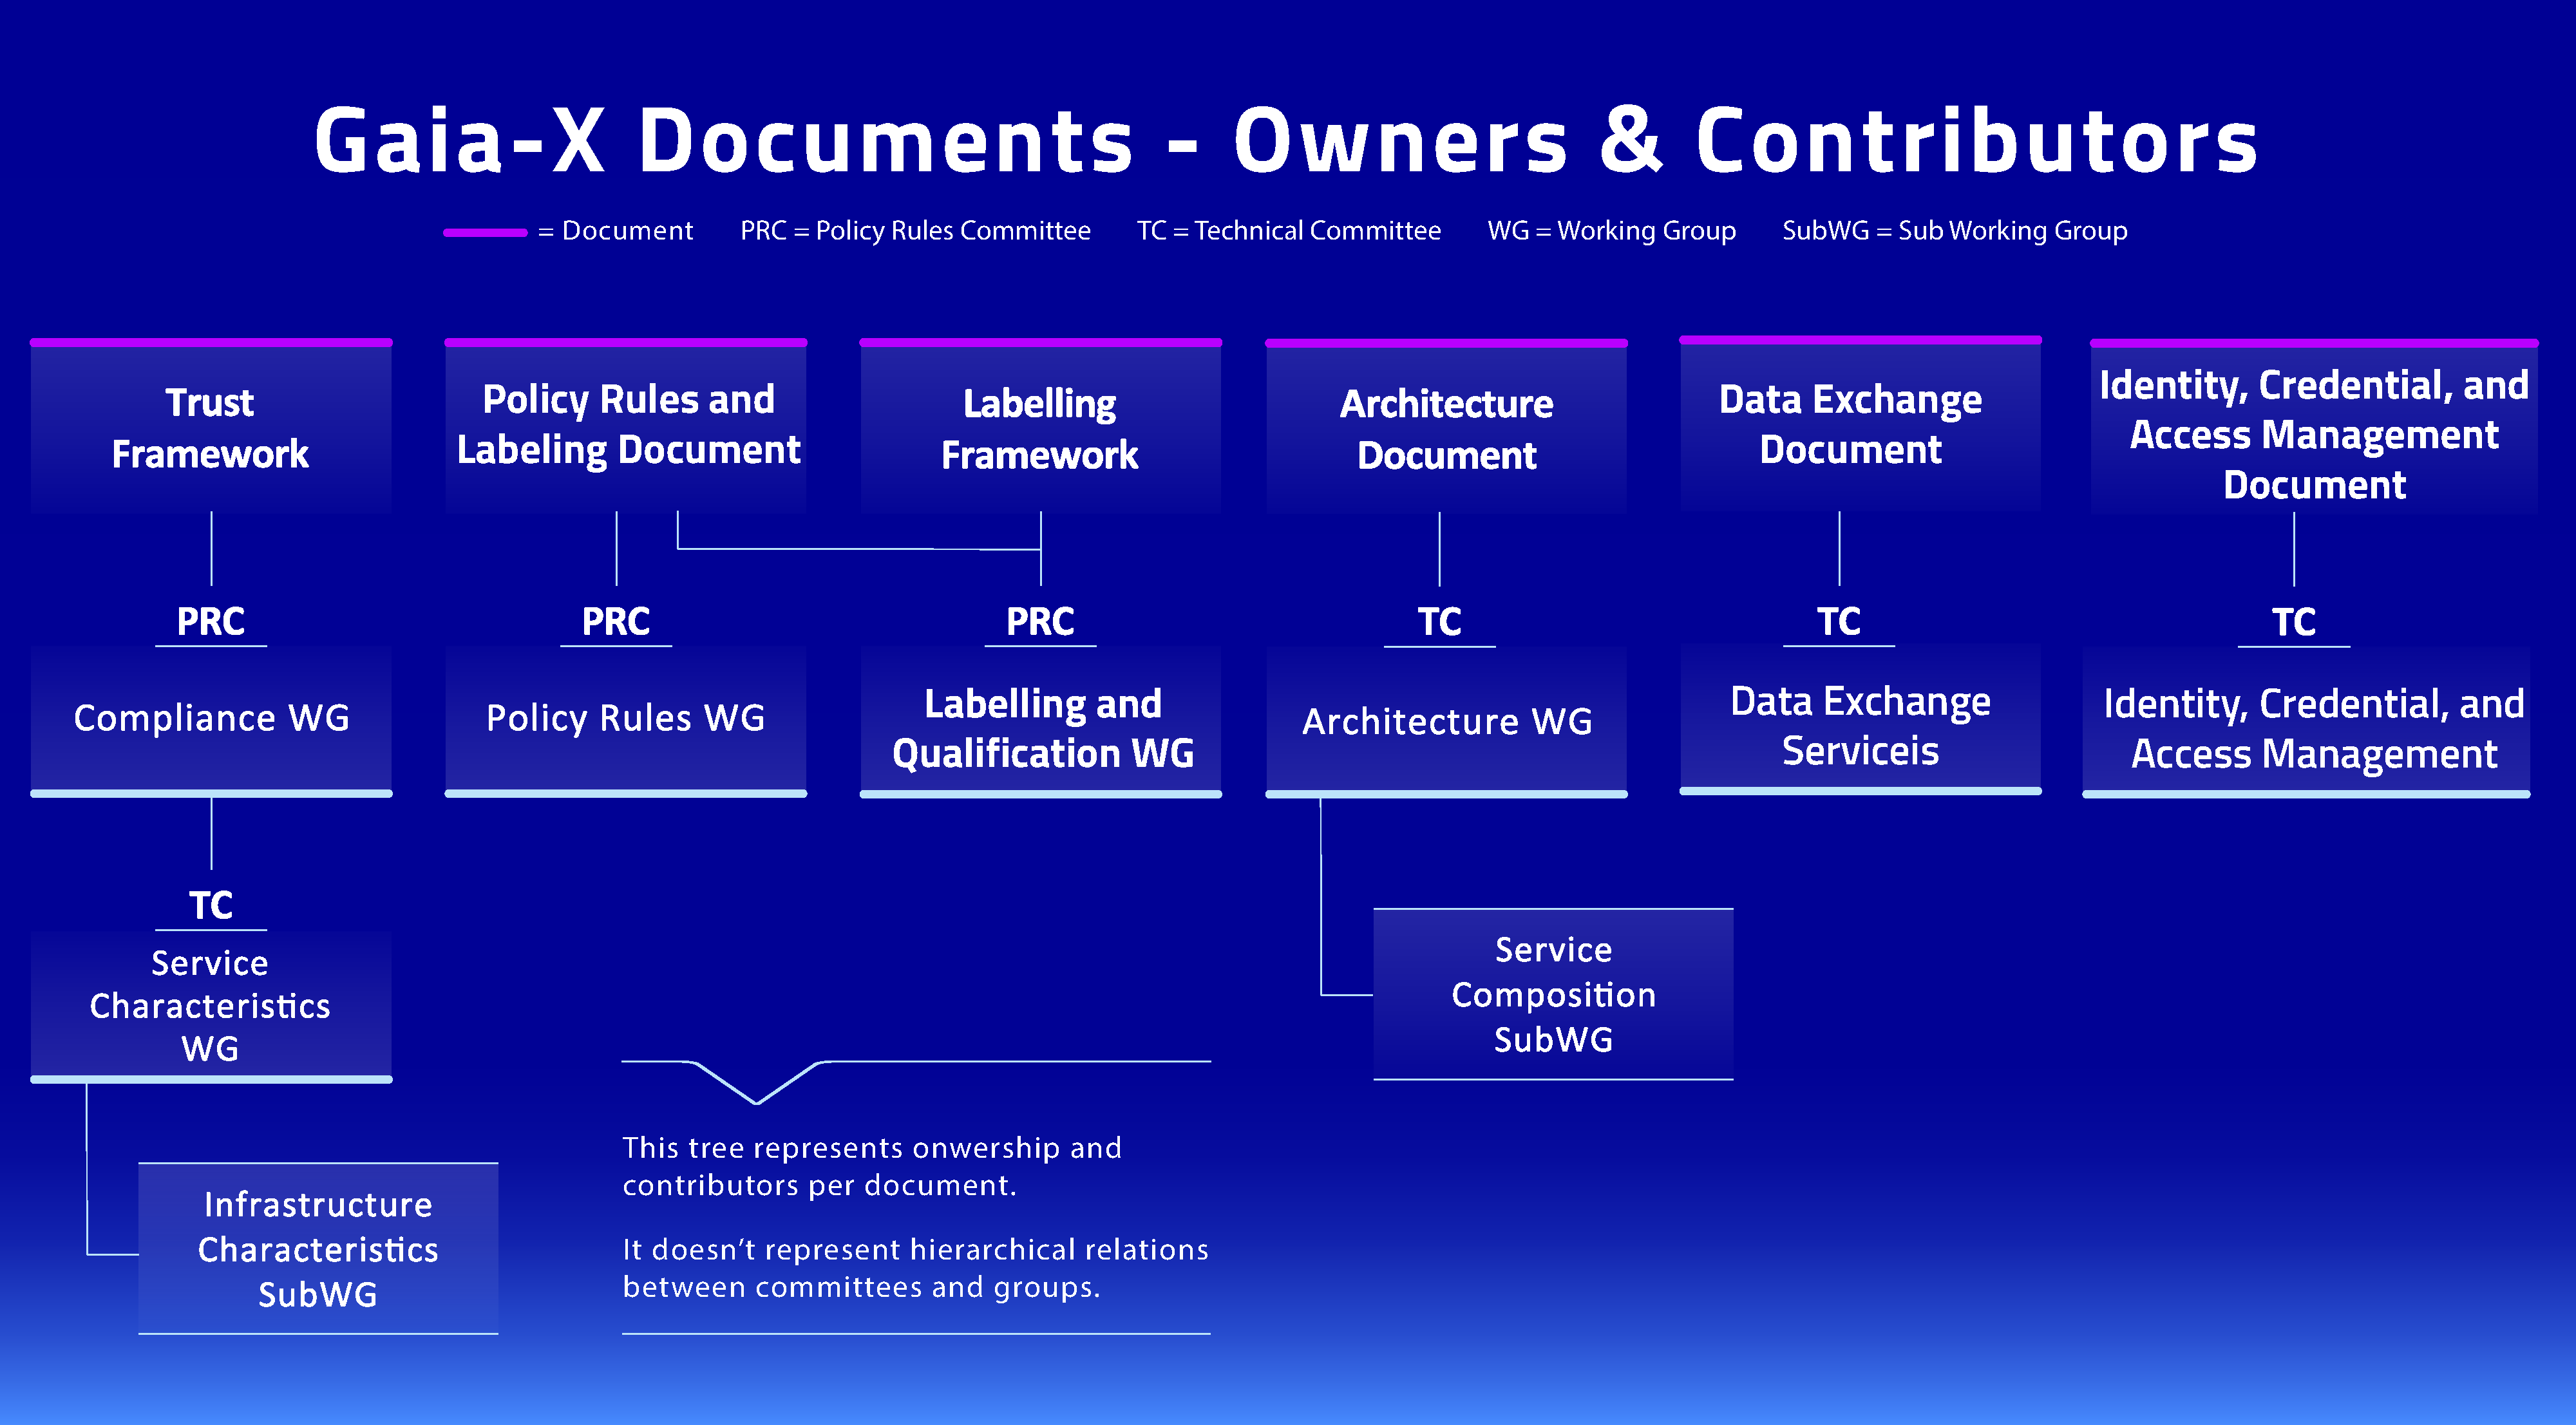
\includegraphics[width=\textwidth]{figures/committees-owners-and-contributors.pdf}
    \caption{Gaia-X Documents - Owners \& Contributors~\cite{gaiax}}\label{fig:gaiax-documents-owners-and-contributors}
\end{figure}

\section{Gaia-X Framework}\label{sec:gaia-x-framework}

Gaia-X Framework (also known as X-Model) is a set of the main deliverable of the initiative and serves to achieve the goal of exchange of digital services, data and cloud storage.
The Gaia-X Association delivers the documents containing formal specifications and requirements for parties wanting to participate in the Gaia-x ecosystem.
These can be categorized into three broad pillars:
\begin{itemize}
    \item Compliance: Decentralized services to enable objective and measurable trust
    \item Federation: Interoperable \& portable Sector or Cross-Sector datasets and services
    \item Data/Service exchange: Anchored contract rules for access and data usage
\end{itemize}

Once the formal specifications are ready, it is the task of the Gaia-X Federation Services (GXFS) project to convert the specifications into freely accessible, open-source software~\cite{gxfs}.
The software is mainly used by Gaia-X participants to support the creation of federations and to provide helpful tools like a logging service or cryptographic libraries.

\begin{figure}
    \centering
    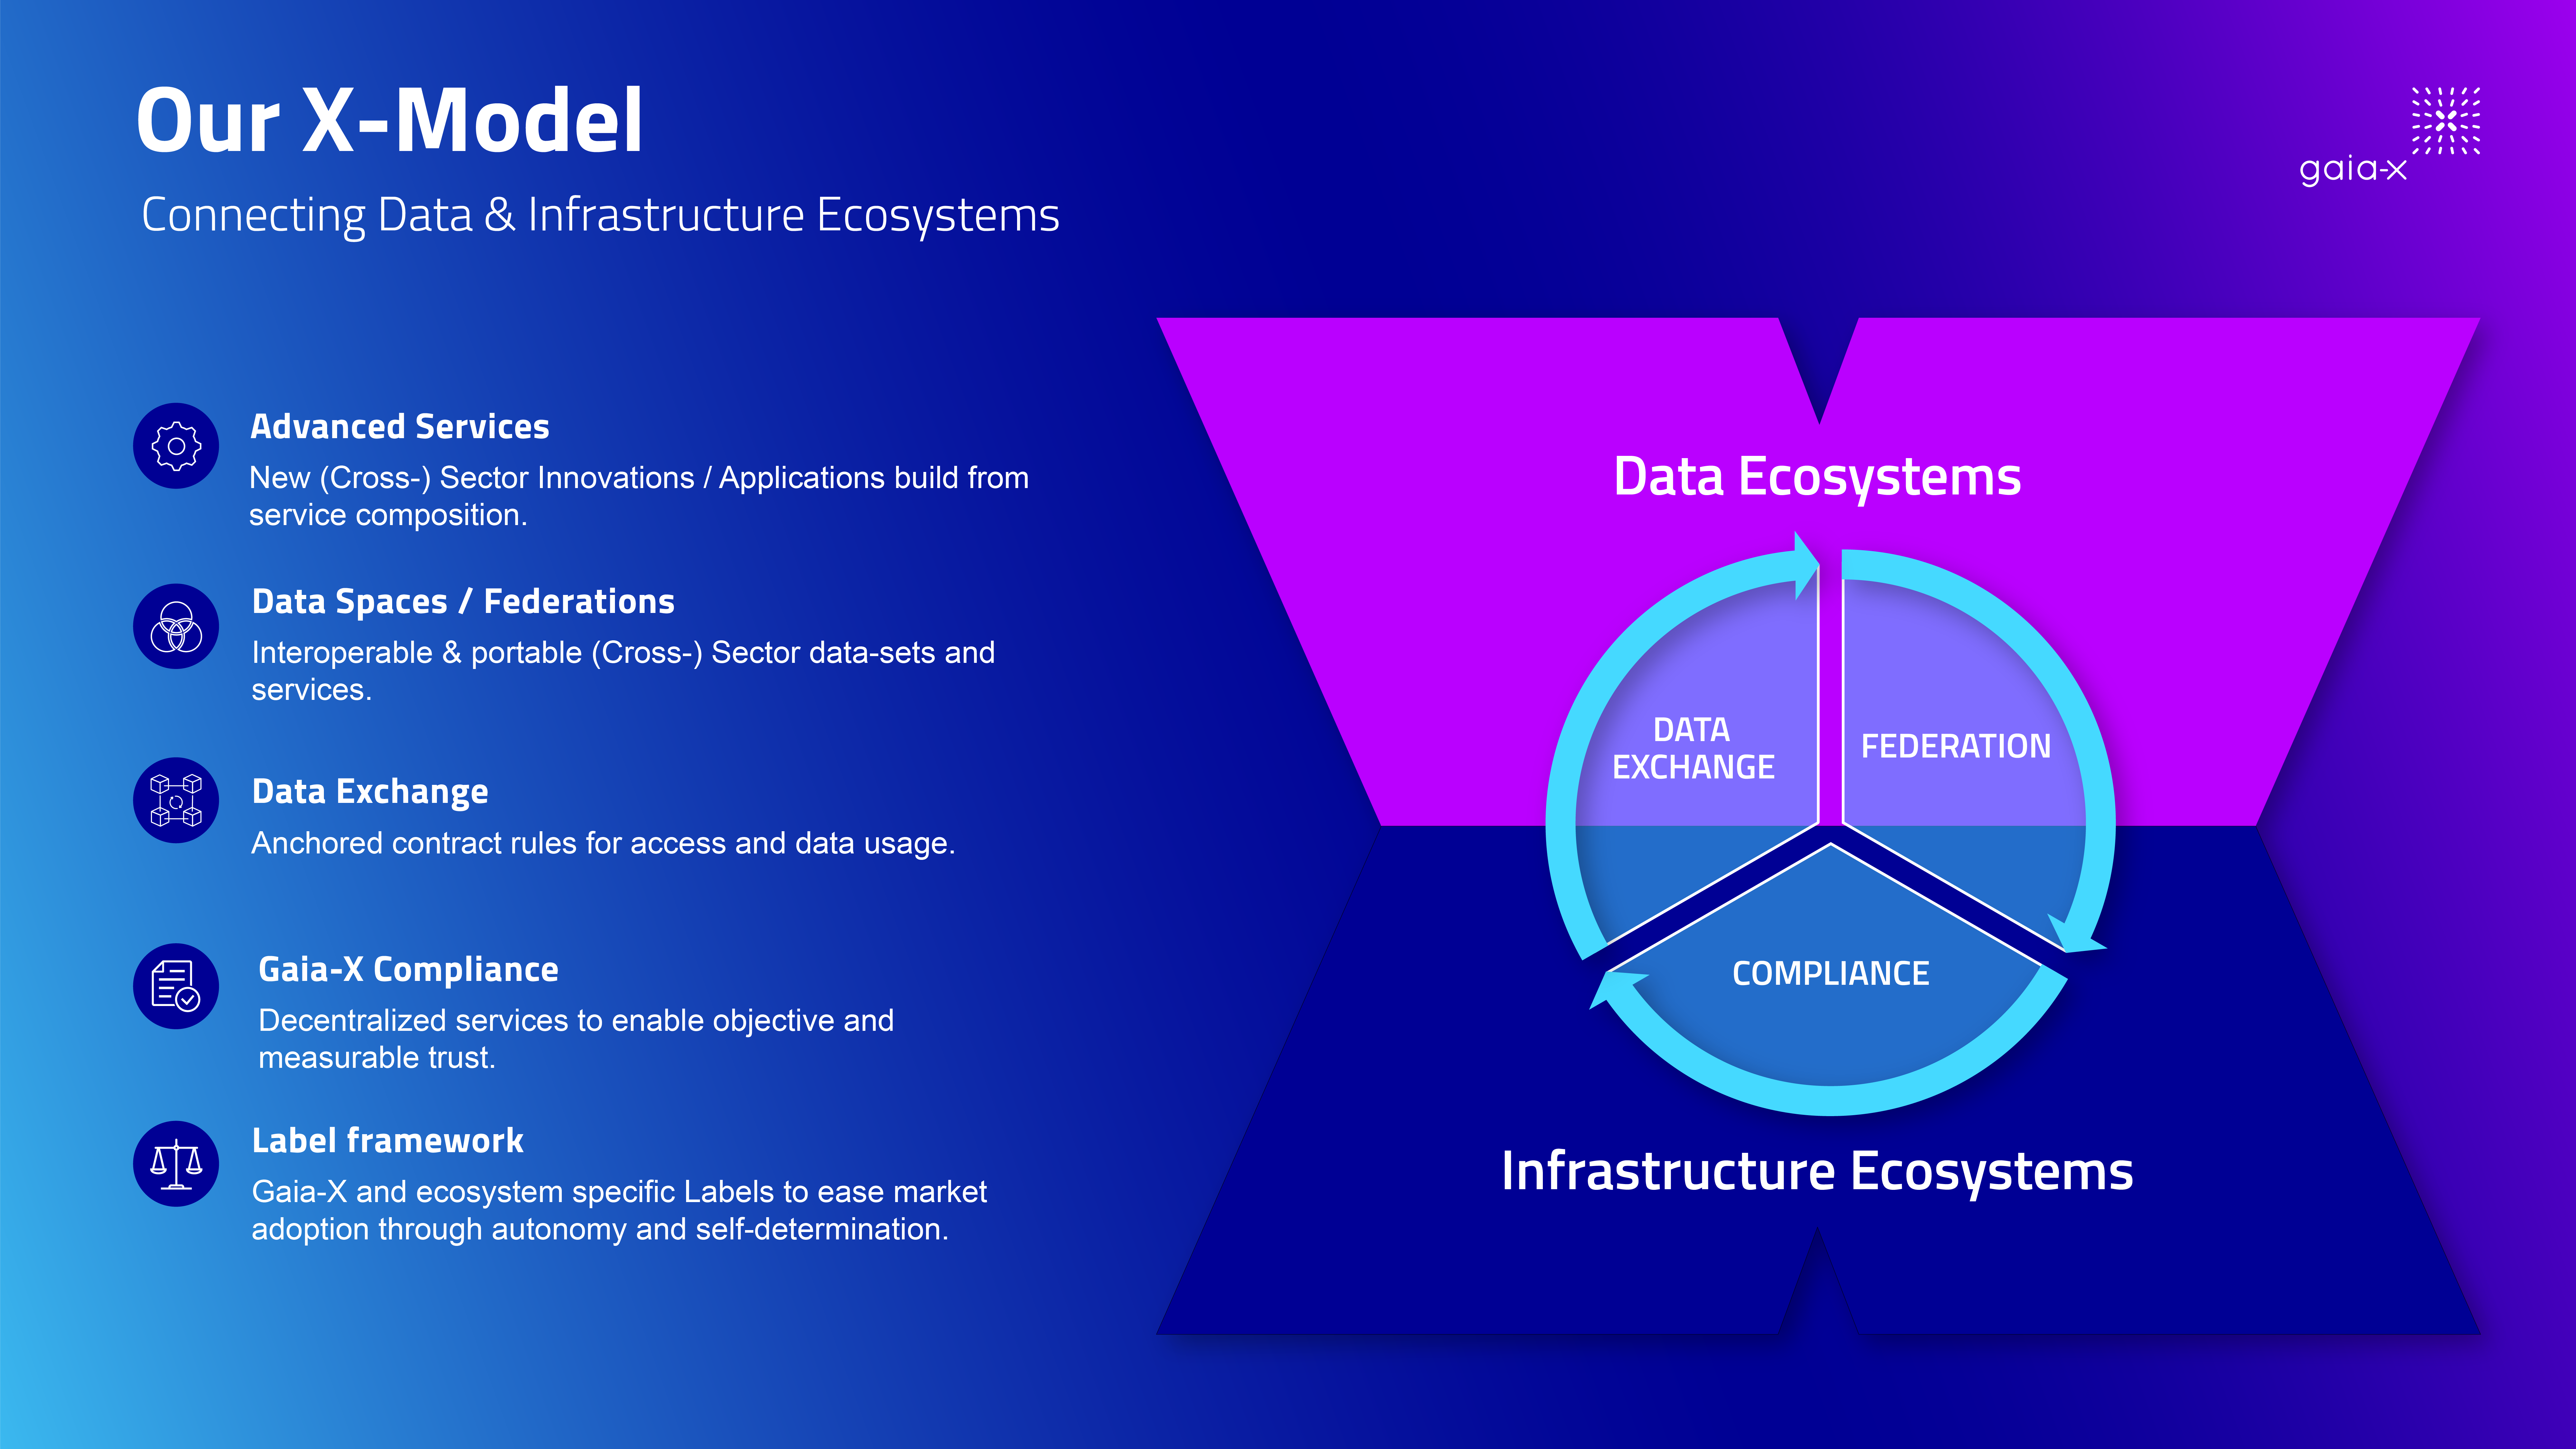
\includegraphics[width=\textwidth]{figures/x-model.png}
    \caption{Gaia-X Framework~\cite{gaiax}}\label{fig:gaiax-x-model}
\end{figure}

\subsection{Policy Rules Conformity Document}\label{subsec:policy-rules-conformity-document}

This document defines high-level objectives of and safeguards the added value and principles of the Gaia-X Ecosystem~\cite{gaiax_policy_rules}.
The policy rules aim to establish clear controls that reflect the core European values of Gaia-X: openness, transparency, data protection, security, and portability.
Basic Conformity sets the minimum requirements for participation in the Gaia-X Ecosystem.
Optional Label levels specify additional criteria and measures, such as certifications, to provide higher assurance and trust, emphasizing European values and complying with EU/EEA legislation.
These initial Labels are expandable, allowing for new Labels to meet sector-specific or regional needs in the future.
Compliance with these policy rules can be demonstrated through adherence to established standards, certifications, and codes of conduct.

The latest version of the document at the time of writing this thesis is 22.10.

\subsection{Architecture document}\label{subsec:architecture-document}

This document outlines the core components of the Gaia-X Trust Framework and explains their interrelationships within the Gaia-X model (see~figure~\ref{fig:gaiax-x-model}) at a functional level~\cite{gaiax_architecture_document}.
Since the Gaia-X Association collaborates with various partners to develop infrastructure and data-driven ecosystems, additionally, this document details how the Gaia-X Trust Framework integrates with implementations of Infrastructure and Data Space-specific services.

The latest version of the document at the time of writing this thesis is 23.10.

\subsection{Trust Framework}\label{subsec:trust-framework}

This document defines the minimum set of rules to be part of the Gaia-X Ecosystem~\cite{gaiax_trust_framework}.
These rules include common governance and basic interoperability across individual ecosystems.
The Gaia-X Trust Framework operationalizes the requirements outlined in Gaia-X documents, such as the Policy Rules, the Labeling Document and the Architecture Document. % FIXME: Labeling document not available on the Gaia-X framework knowlegbase page, reevaluate whether to keep this mention
The latter, in particular, enables federated and interoperable Gaia-X ecosystems.
The framework relies on verifiable credentials and linked data representations as key components for its future operations.

Trusted information must be accessible in machine-readable formats, and when such formats are unavailable, Gaia-X will establish processes to convert this information.
This is essential for federating trusted statements within the Gaia-X ecosystem and for developing mechanisms to reassess the validity of claims within the Trust Framework.
The compliance process, a set of automated and versioned computable rules, ensures this document will also be versioned.
This version of the Gaia-X Trust Framework document supersedes all previous versions.

The latest version of the document at the time of writing this thesis is 22.10.

\subsection{Identity, Credential \& Access Management}\label{subsec:identity-credential-&-access-management}

This document outlines the components of ``Authorization \& Authentication'' that will provide essential functionalities for authorization, access management, and authentication, along with related services, to Gaia-X Participants~\cite{gaiax_identity_and_access_management}.
These functionalities are intended to facilitate participation in the secure environment of the Gaia-X ecosystem.
This document does not address the replacement of an existing IAM System within a Gaia-X participant's environment or its operation therein.

The latest version of the document at the time of writing this thesis is 22.10.

\subsection{Data Exchange services}\label{subsec:data-exchange-services}

This document states the specifications of \textit{Data Exchange Services} including high-level architecture and key requirements for data values, trust and compliance~\cite{gaiax_data_exchange_document}.

The latest version of the document at the time of writing this thesis is 23.11.

\section{Concepts}\label{sec:concepts}

% TODO: explain DID

\subsection{Self-Descriptions}\label{subsec:self-descriptions}
The Gaia-X Framework is centered around so-called \textit{self-descriptions}, which are based on the \textit{W3C Verifiable Credentials Data Model} --- digital, machine-readable credentials containing cryptographical proof from the issuer, in a \textit{JSON-LD} format, which can be linked-up together (e.g., a dataset credential can contain an attribute referencing the credential of the owner of the data).
Self-Descriptions are the cornerstone used to describe all the necessary objects required for participation inside a Gaia-X federation.
These include mainly a \textit{Participant}, \textit{Service Offering} and \textit{Resource}.

\subsection{Ecosystems}\label{subsec:ecosystems}

Gaia-X ecosystems are groups whose goal is to support the creation and development of Data Spaces and projects in different business sectors like Health, Infrastructure, Tourism, etc~\cite{gaiax}. % TODO: define dataspace

The ecosystems aim to create a breeding ground for the creation of new Data Spaces by sharing knowledge, collecting cross-country use-cases and giving Gaia-X Association members the opportunity to network, collaborate and identify open standards related to specific domains.
The cooperation between ecosystems is supported by the Gaia-X Data Space Business Committee to ensure the development and application of Gaia-X deliverables in specific domains.

Currently established ecosystems include the following sectors: Aerospace, Agriculture, Tourism, Education, Energy, Finance, Geoinformation, Health, Manufacturing, Media, Mobility, Public Sector, Smart Cities, Smart Living, Construction and Logistics.

\subsection{Hubs}\label{subsec:hubs}

Apart from Ecosystems, Gaia-X Hubs also exist as groups of companies supporting the needs of Data Spaces~\cite{gaiax}.
Unlike Ecosystems, they act on a regional or country basis.
They serve as the central contact point of contact for interested parties in each country.
They cooperate with the Gaia-X Association in creating expertise and resources, setting up data spaces, and working on use cases.
They can be thought of as think tanks, where concrete data spaces are investigated, designed and implemented.

The hubs are tightly connected to local governments, which allows them to propose solutions in line with the strategic political initiatives and aligned with the goals of the Gaia-X Association and other European hubs~\cite{gaiax}.
In summary, the Gaia-X Hubs have the following objectives:
\begin{itemize}
    \item Act as a local ambassador for Gaia-X
    \item Identify territory specific needs and high priority data spaces
    \item Collaborate with other hubs to develop common pan-European data spaces
    \item Make Gaia-X real identifying projects and creating Gaia-X services in the market
    \item Help local governments implementing RRF in the most effective way adopting Gaia-X solutions
    \item Promote the participation of new members in the association
\end{itemize}
